\documentclass[tikz,border=10pt]{standalone}
\usepackage{tikz}
\usetikzlibrary{positioning, fit, arrows.meta, shapes.geometric, backgrounds, calc}

\begin{document}
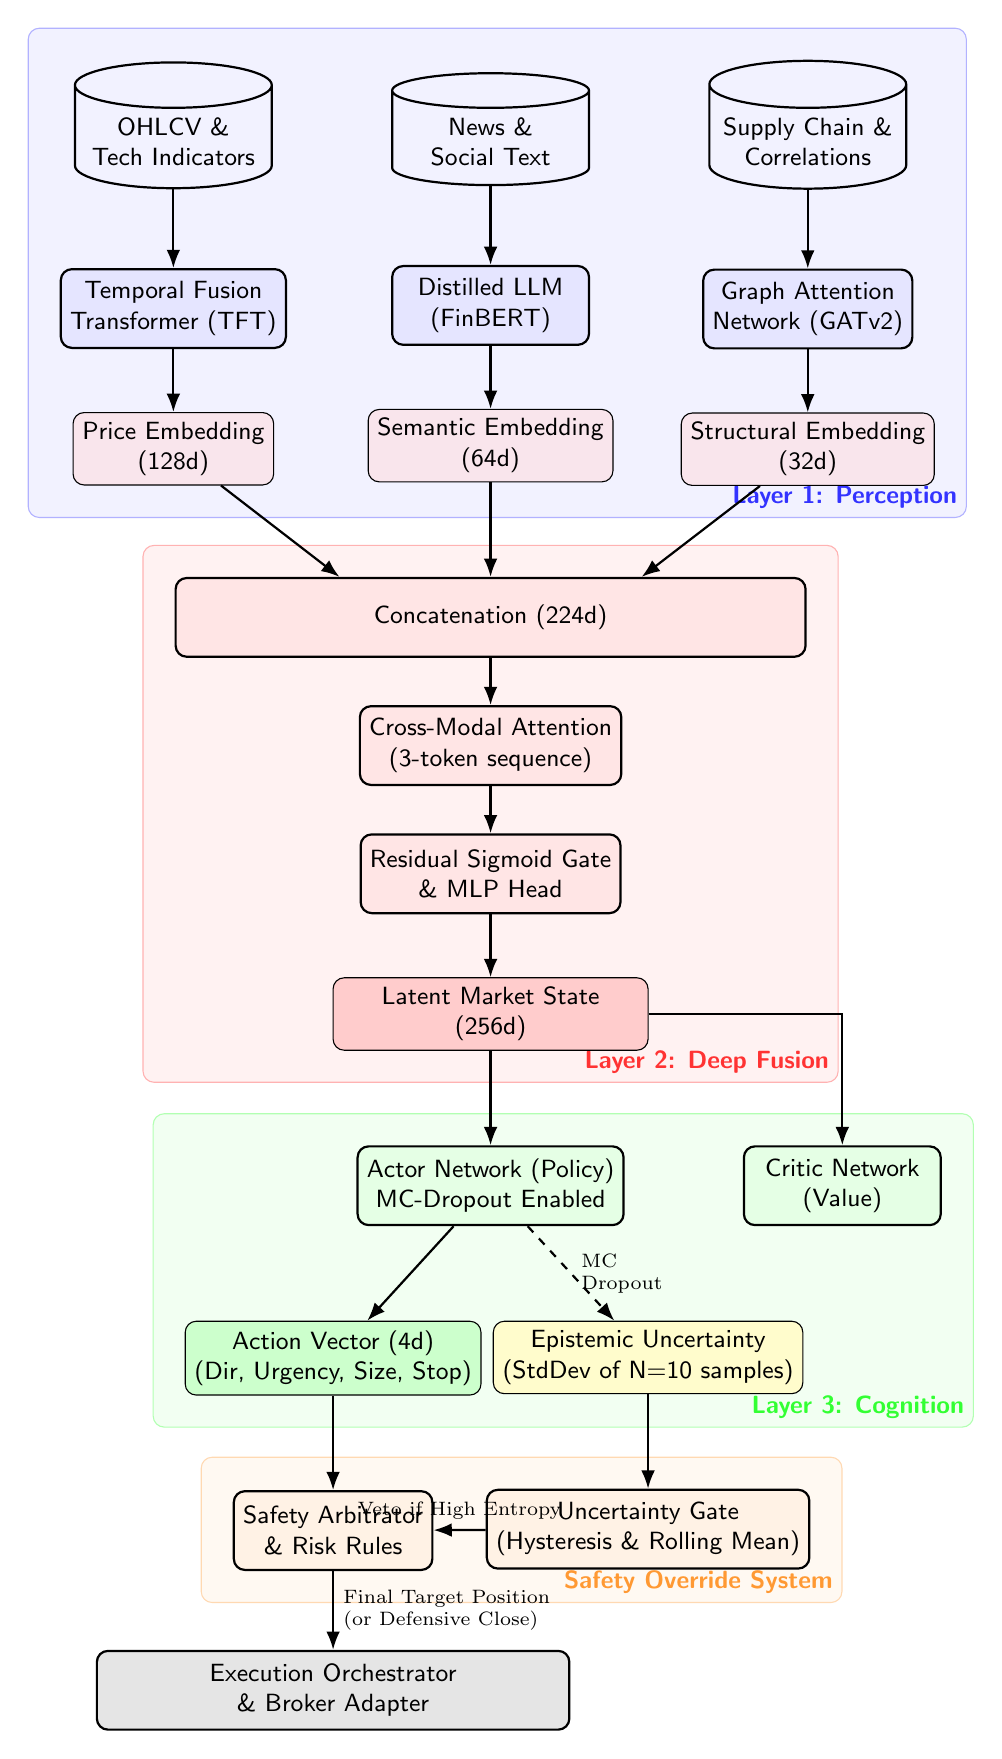
\begin{tikzpicture}[
    font=\sffamily\small,
    >=LaTeX,
    box/.style={rectangle, rounded corners, draw, thick, minimum width=2.5cm, minimum height=1cm, align=center},
    data/.style={cylinder, draw, thick, shape border rotate=90, aspect=0.25, minimum width=2.5cm, minimum height=1cm, align=center},
    encoder/.style={box, fill=blue!10},
    embedding/.style={rectangle, draw, rounded corners, fill=purple!10, minimum height=0.6cm, align=center},
    fusion/.style={box, fill=red!10},
    cognition/.style={box, fill=green!10},
    safety/.style={box, fill=orange!10},
    arrow/.style={->, thick},
    dashed_arrow/.style={->, thick, dashed}
]

% Data Layer
\node[data] (ohlcv) {OHLCV \& \\ Tech Indicators};
\node[data, right=1.5cm of ohlcv] (news) {News \& \\ Social Text};
\node[data, right=1.5cm of news] (graph) {Supply Chain \& \\ Correlations};

% Perception Layer (Encoders)
\node[encoder, below=1cm of ohlcv] (tft) {Temporal Fusion \\ Transformer (TFT)};
\node[encoder, below=1cm of news] (llm) {Distilled LLM \\ (FinBERT)};
\node[encoder, below=1cm of graph] (gnn) {Graph Attention \\ Network (GATv2)};

\draw[arrow] (ohlcv) -- (tft);
\draw[arrow] (news) -- (llm);
\draw[arrow] (graph) -- (gnn);

% Embeddings
\node[embedding, below=0.8cm of tft] (emb_price) {Price Embedding \\ (128d)};
\node[embedding, below=0.8cm of llm] (emb_sem) {Semantic Embedding \\ (64d)};
\node[embedding, below=0.8cm of gnn] (emb_graph) {Structural Embedding \\ (32d)};

\draw[arrow] (tft) -- (emb_price);
\draw[arrow] (llm) -- (emb_sem);
\draw[arrow] (gnn) -- (emb_graph);

% Fusion Layer
\node[fusion, minimum width=8cm, below=1.2cm of emb_sem] (concat) {Concatenation (224d)};
\draw[arrow] (emb_price) -- (concat.165);
\draw[arrow] (emb_sem) -- (concat);
\draw[arrow] (emb_graph) -- (concat.15);

\node[fusion, below=0.6cm of concat] (attn) {Cross-Modal Attention \\ (3-token sequence)};
\draw[arrow] (concat) -- (attn);

\node[fusion, below=0.6cm of attn] (gate) {Residual Sigmoid Gate \\ \& MLP Head};
\draw[arrow] (attn) -- (gate);

\node[embedding, fill=red!20, below=0.8cm of gate, minimum width=4cm] (latent) {Latent Market State \\ (256d)};
\draw[arrow] (gate) -- (latent);

% Cognition Layer
\node[cognition, below=1.2cm of latent] (actor) {Actor Network (Policy) \\ MC-Dropout Enabled};
\node[cognition, right=1.5cm of actor] (critic) {Critic Network \\ (Value)};

\draw[arrow] (latent) -- (actor);
\draw[arrow] (latent) -| (critic);

\node[embedding, fill=green!20, below=1.2cm of actor, xshift=-2cm] (action) {Action Vector (4d) \\ (Dir, Urgency, Size, Stop)};
\node[embedding, fill=yellow!20, below=1.2cm of actor, xshift=2cm] (uncertainty) {Epistemic Uncertainty \\ (StdDev of N=10 samples)};

\draw[arrow] (actor) -- (action);
\draw[dashed_arrow] (actor) -- node[right, font=\scriptsize, align=left] {MC \\ Dropout} (uncertainty);

% Safety & Execution
\node[safety, below=1.2cm of action] (arbitrator) {Safety Arbitrator \\ \& Risk Rules};
\node[safety, below=1.2cm of uncertainty] (unc_gate) {Uncertainty Gate \\ (Hysteresis \& Rolling Mean)};

\draw[arrow] (action) -- (arbitrator);
\draw[arrow] (uncertainty) -- (unc_gate);
\draw[arrow] (unc_gate) -- node[above, font=\scriptsize] {Veto if High Entropy} (arbitrator);

\node[box, fill=gray!20, below=1cm of arbitrator, minimum width=6cm] (broker) {Execution Orchestrator \\ \& Broker Adapter};
\draw[arrow] (arbitrator) -- node[right, font=\scriptsize, align=left] {Final Target Position \\ (or Defensive Close)} (broker);

% Grouping Boxes
\begin{scope}[on background layer]
    \node[draw=blue!30, fill=blue!5, rounded corners, fit=(ohlcv)(news)(graph)(tft)(llm)(gnn)(emb_price)(emb_graph), inner sep=0.4cm] (layer1) {};
    \node[above left, text=blue!80] at (layer1.south east) {\textbf{Layer 1: Perception}};

    \node[draw=red!30, fill=red!5, rounded corners, fit=(concat)(attn)(gate)(latent), inner sep=0.4cm] (layer2) {};
    \node[above left, text=red!80] at (layer2.south east) {\textbf{Layer 2: Deep Fusion}};

    \node[draw=green!30, fill=green!5, rounded corners, fit=(actor)(critic)(action)(uncertainty), inner sep=0.4cm] (layer3) {};
    \node[above left, text=green!80] at (layer3.south east) {\textbf{Layer 3: Cognition}};

    \node[draw=orange!30, fill=orange!5, rounded corners, fit=(arbitrator)(unc_gate), inner sep=0.4cm] (layer4) {};
    \node[above left, text=orange!80] at (layer4.south east) {\textbf{Safety Override System}};
\end{scope}

\end{tikzpicture}
\end{document}
